\section{What are the redundant files?}
\label{sec:redundant_files}

\begin{table} 
	\centering 
	\scriptsize  
	%\begin{minipage}{.5\linewidth}
	\caption{Summary of file \& dir. characterization} \label{tbl:sum_file_dir_char} 
	\begin{tabular}{|l|l|l|l|l|}%p{0.14\textwidth} 
		\hline 
		% after \\: \hline or \cline{col1-col2} \cline{col3-col4} ... 
		% after \\: \hline or \cline{col1-col2} \cline{col3-col4} ... 
		Metrics & max & min & median & avg.\\
		\hline
		File size &   &   &   &  \\
		\hline
		File size (repeat cnt. $>$ 1) &   &   &    &  \\
		\hline
		File size (repeat cnt. $=$ 1) &   &   &    &  \\
		\hline
		\hline
		Dir. size &  &  & & \\
		\hline
		File cnt. per dir & &  &  & \\
		\hline
		Redundant ratio & &  &  & \\
		\hline
		Dir. depth  &  &  & & \\
		\hline
	\end{tabular} 
\end{table} 

\subsection{Redundant file storage overhead analysis}

\paragraph{Cumulative distribution and probability distribution of file repeat count}

Almost 90\% of files have equal or less than 10 redundant copies. Most files have small repeat count.

\begin{figure}
	\centering
	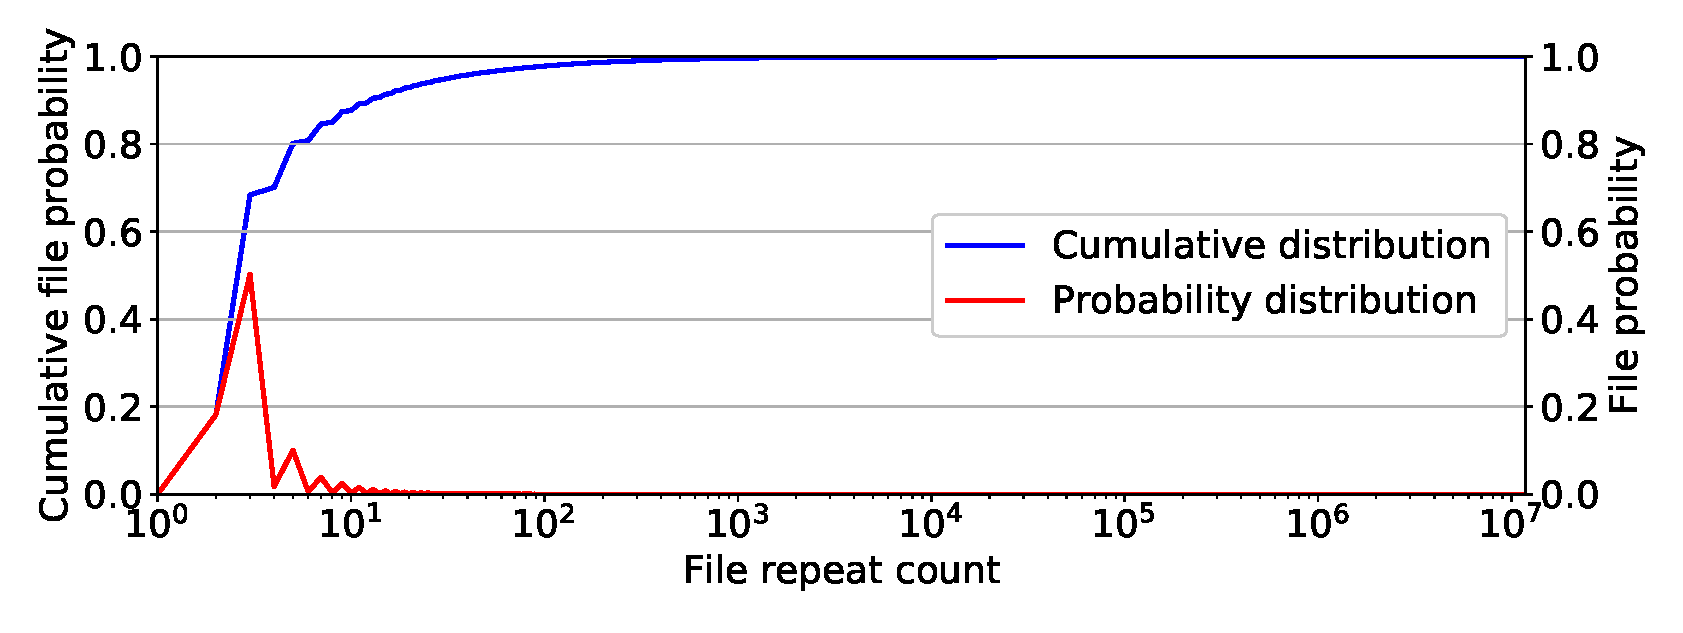
\includegraphics[width=0.5\textwidth]{graphs/File_repeat_count.eps}
	\caption{CDF of file repeat count.
	}
	\label{fig:file_repeat_count}
\end{figure}

\paragraph{Cumulative distribution and probability distribution of file size in terms of unique file size, redundant file size, overall file size}

91\% files'sizes are equal or less than 100KB. Most files are smaller files.

\begin{figure}
	\centering
	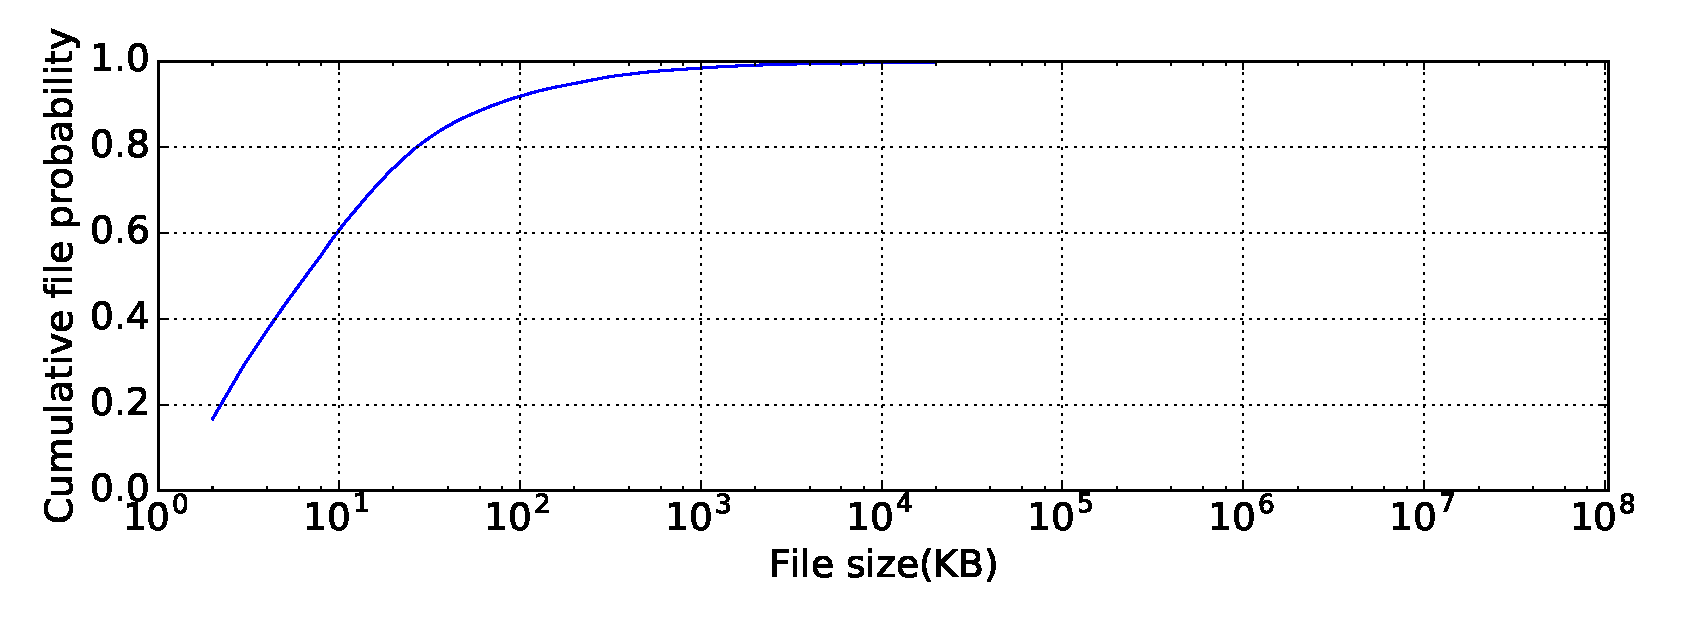
\includegraphics[width=0.5\textwidth]{graphs/File_size-KB.eps}
	\caption{CDF of unique file size (KB).
	}
	\label{fig:file_size}
\end{figure}

%\paragraph{Average file size by repeat count}
%
%There is no relation between file repeat count and average file size.
%
%\begin{figure}
%	\centering
%	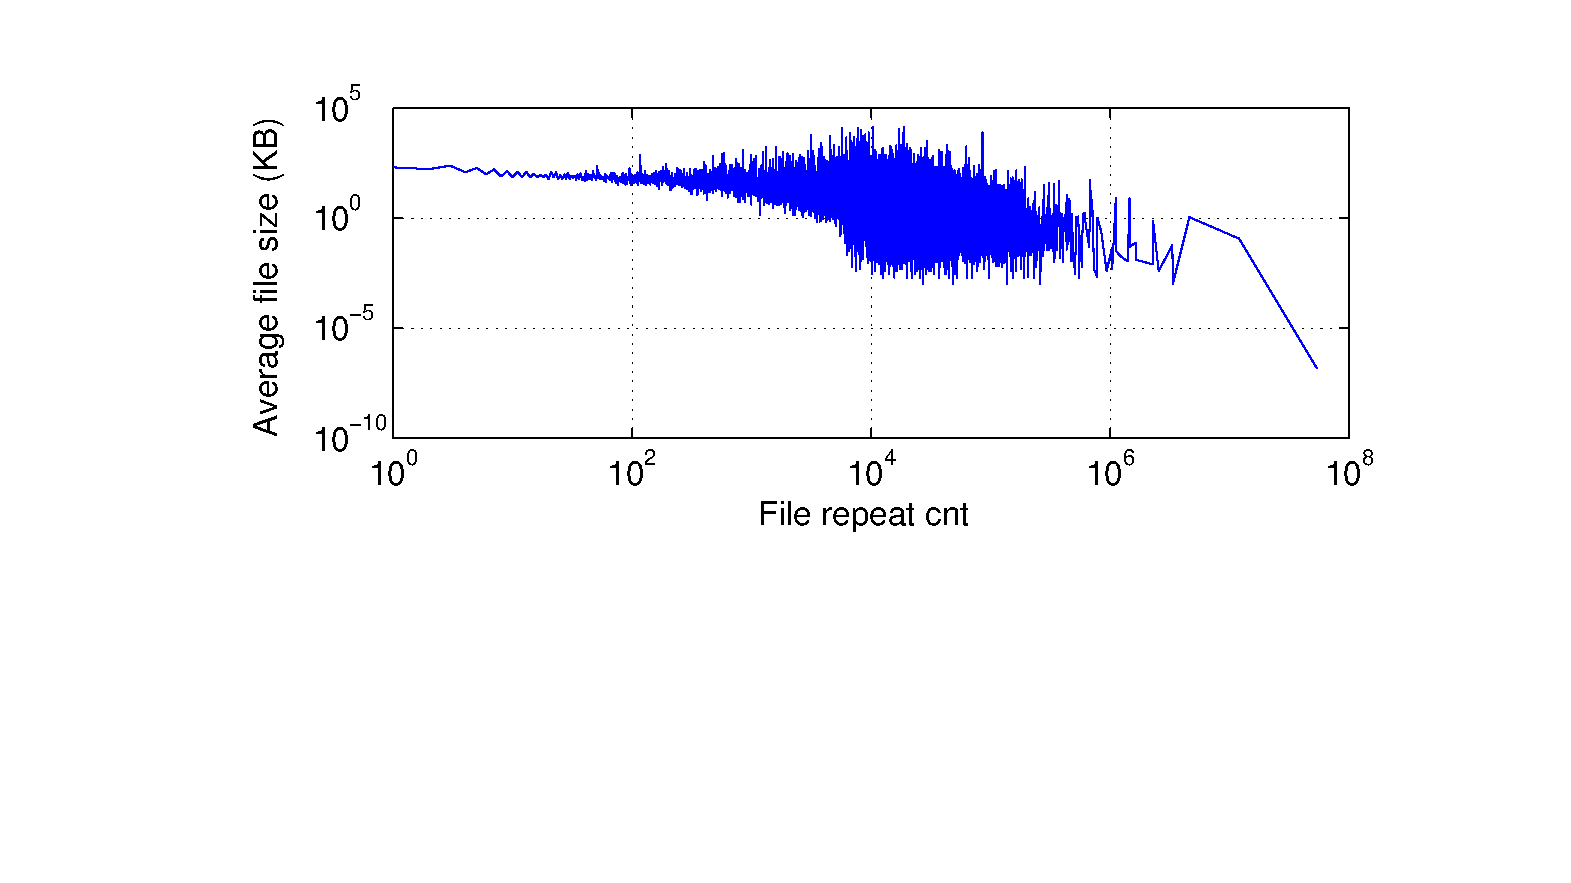
\includegraphics[width=0.5\textwidth]{graphs/avg_size_by_cnt.eps}
%	\caption{Average file size with same repeat count.
%	}
%	\label{fig_avg_size_by_cnt}
%\end{figure}
%
%\paragraph{Redundant ratio by file size for the files with the same content in terms of file count and storage capacity}
%Total size of redundant files with same content(TRS)
%
%97\% of the TRSs are equal or less than 100MB.
%
%\begin{figure}
%	\centering
%	\includegraphics[width=0.5\textwidth]{graphs/Total_size_of_redudant_files_with_same_content-KB.eps}
%	\caption{CDF of total file size with same file content (MB).
%	}
%	\label{fig_total_redundant_same_digest}
%\end{figure}
%
%\paragraph{Redundant ratio by repeat count for the files with the same repeat count in terms of file count and storage capacity}
%
%However, with the increase of file repeat count, the sum of file size with same repeat count becomes smaller.
%
%\begin{figure}
%	\centering
%	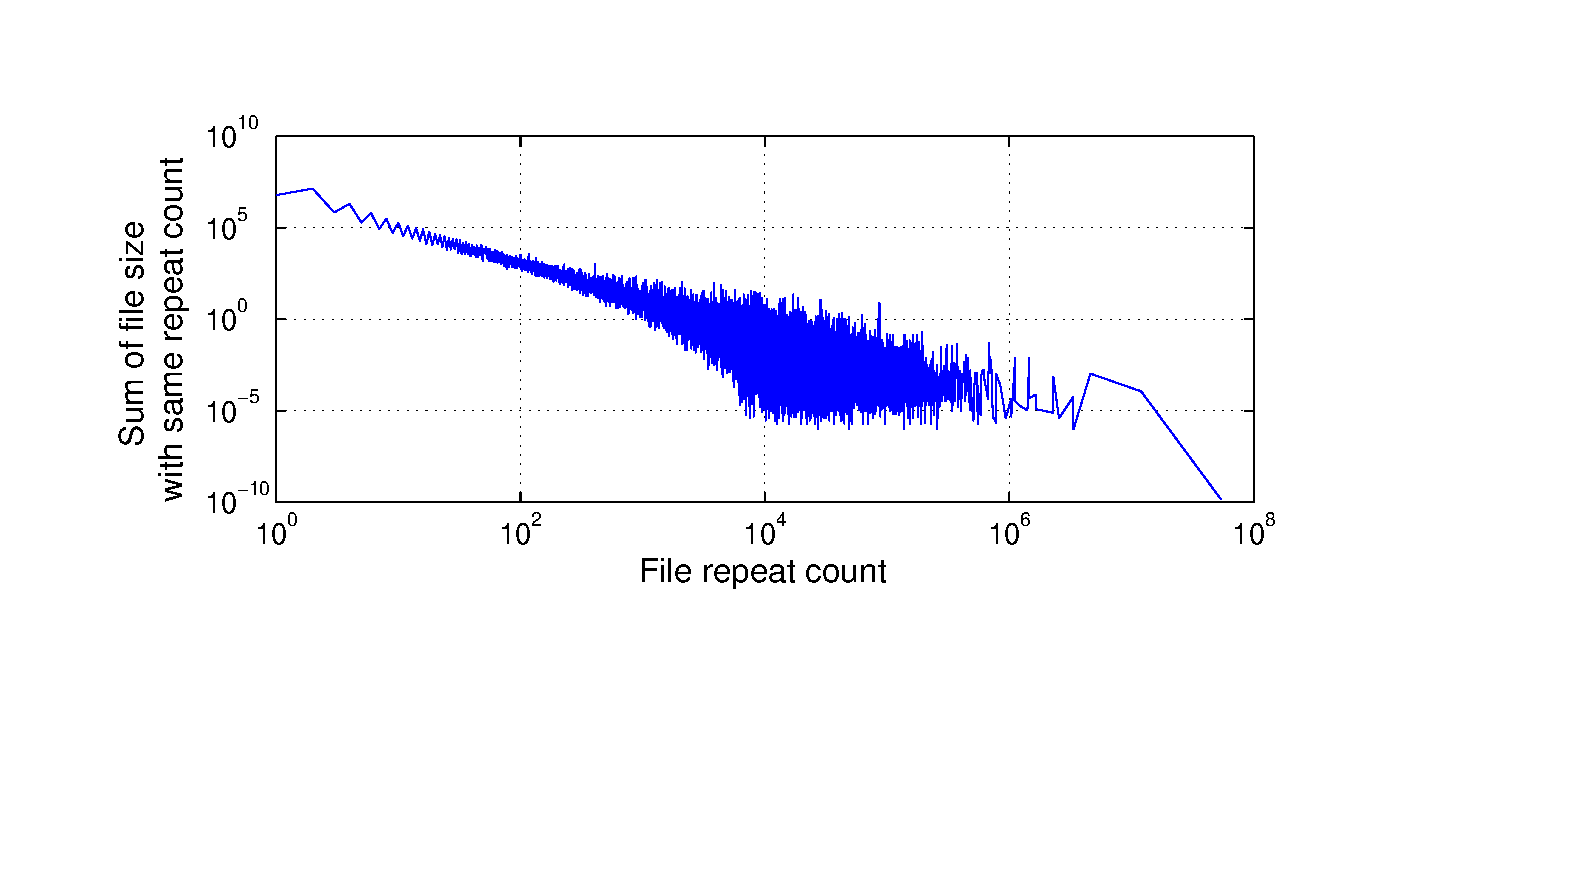
\includegraphics[width=0.5\textwidth]{graphs/sum_size_by_cnt.eps}
%	\caption{Sum of file size with same repeat count.
%	}
%	\label{fig_sum_by_cnt}
%\end{figure}

\subsection{Redundant file characterization}


\begin{table} 
	\centering 
	\scriptsize  
	\caption{Top 20 redundant files' characterization (sorted by repeat cnt.)}
	\label{tbl:top_dup_files_repeat_cnt} 
	\begin{tabular}{|l|l|l|l|l|}%p{0.14\textwidth} 
		\hline 
		Filename & repeat cnt. & type & extension & size \\
		\hline
		&   &   &   &  \\
		\hline
		&   &   &   &   \\
		\hline
		&   &   &  &    \\
		\hline
		&  &  &  & \\
		\hline
		& &  &   & \\
		\hline
		& &  &   & \\
		\hline
		&  &  & & \\
		\hline
	\end{tabular} 
\end{table}

\begin{table} 
	\centering 
	\scriptsize  
	\caption{Top 20 redundant files' characterization (sorted by capacity)} 
	\label{tbl:top_dup_files_cap} 
	\begin{tabular}{|l|l|l|l|l|}%p{0.14\textwidth} 
		\hline 
		Filename & repeat cnt. & type & extension & size \\
		\hline
		&   &   &   &  \\
		\hline
		&   &   &   &   \\
		\hline
		&   &   &  &    \\
		\hline
		&  &  &  & \\
		\hline
		& &  &   & \\
		\hline
		& &  &   & \\
		\hline
		&  &  & & \\
		\hline
	\end{tabular} 
\end{table}


\begin{table} 
	\centering 
	\scriptsize  
	\caption{Top redundant file types} 
	\label{tbl:top_dup_types} 
	\begin{tabular}{|l|l|l|l|l|l|}%p{0.14\textwidth} 
		\hline 
		Type & extension & Num. & size & red. ratio (cnt.)  & red. ratio (cap.)\\
		\hline
		  &   &   &  & &   \\
		\hline
		  &   &   &  & &    \\
		\hline
		  &   &   &   & &   \\
		\hline
		 &  &  &  & & \\
		\hline
		  & &  &  & & \\
		\hline
		  & &  & & &  \\
		\hline
		   &  &  & & &  \\
		\hline
	\end{tabular} 
\end{table} 

